%\title{Appendix: Worst-case Optimal Submodular Extensions for Marginal Estimation}
\appendix
\mysection{Proofs for Potts Model Extension} 

\paragraph{Remark 1} We show using induction over the number of variables that with $1$-of-$L$ encoding for Potts, 

\begin{equation}
    \sum_{A \in {\mathcal M}} \exp(-s(A)) = \prod_{a = 1}^{N} \sum_{i = 1}^L \exp(-s_{ai})
    \label{eq:ind}
\end{equation}

\begin{proof}
Let $t$ be the number of variables, $V^t$ be the corresponding ground set and ${\mathcal M}^t$ be the sets corresponding to valid labelings. Equation \eqref{eq:ind} clearly holds for $t = 1$.

Let us assume that the relation holds for $t = N$, that is,

\begin{equation}
    \sum_{A^N \in {\mathcal M}^N} \exp(-s(A^N)) = \prod_{a = 1}^{N} \sum_{i = 1}^L \exp(-s_{ai})
\end{equation}

For $t = N + 1$, 

\begin{align}
    \sum_{A^{N + 1} \in {\mathcal M}^{N + 1}} \exp(-s(A^{N + 1})) &=  \sum_{i = 1}^L \sum_{A^N \in {\mathcal M}^{N}} \exp(-s(A^N) - s_{N+1, i}) \nonumber \\
                                                                  &= \sum_{i = 1}^L \exp(-s_{N+1, i}) \sum_{A^N \in {\mathcal M}^{N}} \exp(-s(A^N) ) \nonumber \\
                                                                  &= \sum_{i = 1}^L \exp(-s_{N+1, i}) \prod_{a = 1}^{N} \sum_{i = 1}^L \exp(-s_{ai}) \nonumber \\
                                                                  &= \prod_{a = 1}^{N + 1} \sum_{i = 1}^L \exp(-s_{ai})
\end{align}
\end{proof}
{\lemma Given any submodular extension $F(.)$ of a Potts energy function $E(.)$, its Lovasz extension $f(.)$ defines an LP relaxation of the MAP problem for $E(.)$ as 
\begin{align}
    \min_{{\bf y} \in \Delta} f({\bf y}).
\end{align}
%\label{lemma:lovasz_lp}}
\begin{proof}
    By definition of a submodular extension and the Lovasz extension, $E({\bf x}) = F(A_{\bf x}) = f(1_{A_{\bf x}})$ for all valid labelings ${\bf x}$. Also, from property 1, $f({\bf y})$ is maximum of linear functions. Hence, $f({\bf y})$ is a piecewise linear relaxation of $E({\bf x})$.

    The domain $\Delta$ is a polytope formed by union of $N$ probability simplices
\begin{equation}
    \Delta = \{{\bf y}_a \in \mathbb{R}^L | {\bf y}_a \succeq 0  \textrm{ and } \langle {\bf 1}, {\bf y}_a \rangle = 1\}
\end{equation}
With objective as maximum of linear functions and domain as a polytope, we have an LP relaxation of the corresponding MAP problem.
\end{proof}

\mysection{Proofs for Hierarchical Potts Model Extension} 
\myparagraph{Transformed Tightest LP Relaxation} We take (T-LP) and rewrite it using indicator variables for all labels and meta-labels. Let $\mathcal R$ denote the set of all labels and meta-labels, that is, all nodes in the tree apart from the root. Also, let $\mathcal L$ denote the set of labels, that is, the leaves of the tree. Let $T_i$ denote the subtree which is rooted at the $i$-th node. We introduce an indicator variable $z_{ai} \in \{0, 1\}$, where
\begin{align}
    \enskip  z_{ai} =  \begin{cases} 
        y_{ai} \quad &\text{if} \enskip i \in {\mathcal L} \\
        y_{a}(T_i) \quad &\text{if} \enskip i \in {\mathcal R - \mathcal L} \\
    \end{cases}
\end{align}

We need to extend the definition of unary potentials to the expanded label space as follows:
\begin{align}
    \text{where} \enskip    \phi'_{a}(i) =  \begin{cases} 
        \phi_{a}(i) \quad &\text{if} \enskip i \in {\mathcal L} \\
        0  \quad &\text{if} \enskip i \in {\mathcal R - L} \\
    \end{cases}
\end{align}
%
We can now rewrite problem \eqref{eq:t-lp} in terms of new indicator variables $z_{ai}$:
%
\begin{align}
    \text{(T-LP-FULL)} \quad &\min \widetilde{E}({\bf z}) = \sum_{i \in \mathcal{R}} \sum_{a \in {\mathcal X}} \phi_a'(i) \cdot z_{ai} + \nonumber \\
            &\sum_{i \in \mathcal{R}} \sum_{(a, b) \in {\mathcal N}} w_{ab} \cdot l_{T_i} \cdot |z_{ai} - z_{bi}| \nonumber \\
    \text{such that} \quad {\bf z} \in \Delta'
%\label{eq:t-lp-full}
\end{align}
   where $\Delta'$ is the convex hull of the vectors satisfying
\begin{align}
    \enskip &\sum_{i \in \mathcal{L}} z_{ai} = 1, \enskip z_{ai} \in \{0, 1\} \enskip \forall a \in {\mathcal X}, i \in \mathcal{L} \\
    \text{and} \enskip &z_{ai} = \sum_{j \in L(T_i) } z_{aj}.\enskip \forall a \in {\mathcal X}, i \in \mathcal{R - L} %\label{eq:consistency_constraint} 
\end{align}
%
Constraint (\ref{eq:consistency_constraint}) ensures consistency among labels and meta-labels, that is, if a label is assigned then all the meta-labels which lie on the path from the root to the label should be assigned as well. We are now going to identify a suitable set encoding and the worst-case optimal submodular extension using (T-LP-FULL).


{\lemma Given any submodular extension $F(.)$ of an hierachical Potts energy function $E(.)$, its Lovasz extension $f(.)$ defines an LP relaxation of the corresponding MAP estimation problem as
\begin{align}
    \min_{{\bf z} \in \Delta'} f({\bf z}) 
\end{align}
%\label{lemma:lovasz_lp_metric}}

\begin{proof}
    By definition of a submodular extension and the Lovasz extension, $E({\bf x}) = F(A_{\bf x}) = f(1_{A_{\bf x}})$ for all valid labelings ${\bf x}$. Also, from property 1, $f({\bf y})$ is maximum of linear functions. Hence, $f({\bf y})$ is a piecewise linear relaxation of $E({\bf x})$.

    We can write the domain $\Delta'$ as 
    \begin{equation}
    \Delta' = \{ {\bf y}_a \in \mathbb{R}^M | {\bf y}_a \succeq 0, \enskip \langle {\bf 1}, {\bf y}_a^{label} \rangle = 1, \enskip {\bf y}_a(p_{ai}) = {\bf 1} \textrm{ or } {\bf y}_a(p_{ai}) = {\bf 0} \forall i \in [1, L]\}
    \end{equation} 
where ${\bf y}_a$ is the component of $\bf y$ corresponding to the $a$-th variable, ${\bf y}_a^{label}$  is the component of ${\bf y}_a$ corresponding to the $L$ labels, and ${\bf y}_a(p_{ai})$ is the component of ${\bf y}_a$ corresponding to the elements of $p_{ai}$. 

    Since $\Delta'$ is defined by linear equalities and inequalities, it is a polytope. With objective as maximum of linear functions and domain as a polytope, we have an LP relaxation of the corresponding MAP problem.
\end{proof}


{\proposition In the limit $T \to 0$, the following problem for hierarchical Potts energies 

\begin{equation}
\min_{{\bf s} \in EP(F)} \quad g_T ({\bf s}) = \sum_{a = 1}^{N} T \cdot \log \sum_{i = 1}^L \exp(-\frac{s'_{ai}}{T}).
%\label{eq:metric_temp}
\end{equation}
becomes:
\begin{align}
    - \min_{{\bf z} \in \Delta'} f({\bf z}) 
\end{align}
%\label{proposition:metric_equiv}}

\begin{proof}
In the limit of $T \to 0$, we can rewrite the above problem as
\begin{equation}
    \min_{{\bf s} \in EP(F)} \quad \sum_{a = 1}^{N} \max_{i} (-s'_{ai}).
\end{equation}
In vector form, the problem becomes
\begin{align}
    &\min_{{\bf s} \in EP(F)} \max_{{\bf z} \in \Delta} - \langle {\bf z}, {\bf s'} \rangle \\
    & = - \max_{{\bf s} \in EP(F)} \min_{{\bf z} \in \Delta} \langle {\bf z}, {\bf s'} \rangle
    %\label{eq:metric_maxmin}
\end{align}
\begin{equation}
    \text{where } \Delta = \{{\bf z}_a \in \mathbb{R}^L | {\bf z}_a \succeq 0  \textrm{ and } \langle {\bf 1}, {\bf z}_a \rangle = 1\}
\end{equation}
where ${\bf z}_a$ is the component of $\bf z$ corresponding to the $a$-th variable. We can unpack $\bf s'$ using 
\begin{equation}
s'_{ai} = \sum_{t \in p_{ai}} s_t.
%\label{eq:tree_s}
\end{equation}
and rewrite problem \eqref{eq:metric_maxmin} as
\begin{align}
    - \max_{{\bf s} \in EP(F)} \min_{{\bf y} \in \Delta'} \langle {\bf y}, {\bf s} \rangle
    %\label{eq:metric_maxmin_unpack}
\end{align}
The new constraint set $\Delta'$ ensures that the binary entries of labels and meta-labels is consistent:
\begin{align}
    \textrm{where } \Delta' &= \{ {\bf y}_a \in \mathbb{R}^M | {\bf y}_a \succeq 0, \enskip \langle {\bf 1}, {\bf y}_a^{label} \rangle = 1, \nonumber \\
    &\enskip {\bf y}_a(p_{ai}) = {\bf 1} \textrm{ or } {\bf y}_a(p_{ai}) = {\bf 0} \forall i \in [1, L]\}
\end{align} 
where ${\bf y}_a$ is the component of $\bf y$ corresponding to the $a$-th variable, ${\bf y}_a^{label}$  is the component of ${\bf y}_a$ corresponding to the $L$ labels, and ${\bf y}_a(p_{ai})$ is the component of ${\bf y}_a$ corresponding to the elements of $p_{ai}$. 

By the minimax theorem for LP, we can reorder the terms:
\begin{equation}
    - \min_{{\bf y} \in \Delta'} \max_{{\bf s} \in EP(F)} \langle {\bf y}, {\bf s} \rangle 
    %\label{eq:metric_minmax}
\end{equation}
Recall that $\max_{{\bf s} \in EP(F)} \langle {\bf y}, {\bf s} \rangle$ is the value of the Lovasz extension of $F$ at $\bf y$, that is, $f({\bf y})$. Hence, as $T \to 0$, the marginal inference problem converts to minimising the Lovasz extension under the constraints $\Delta'$:
\begin{equation}
    - \min_{{\bf y} \in \Delta'} f({\bf y}) 
    %\label{eq:metric_minLovasz}
\end{equation}
\end{proof}

{\proposition The objective function $\widetilde{E}({\bf z})$ of (T-LP-FULL) is the Lovasz extension of $F_{r-\textrm{HST}}(A) = \sum_{i = 1}^M F_i(A)$, where
\begin{align}
    F_i(A) &= \sum_a \phi'_{a}(i) [|A \cap \{v_{ai}\}| = 1] + \nonumber \\
           &\sum_{(a, b) \in {\mathcal N}} {w_{ab}} \cdot l_{T_i} \cdot [|A \cap \{v_{ai}, v_{bi}\}| = 1]
\end{align}
%\label{proposition:rhst_optimal}}
\begin{proof}
    We observe that $F_{r-\textrm{HST}}$ is of exactly the same form as $F_{Potts}$, except that the Ising models $F_i$ are defined over not just labels, but meta-labels as well. Using the same logic as in the proof of proposition \ref{proposition:a-potts_optimal}, each $F_i$ is the Lovasz extension of 
        \begin{equation}
            \widetilde{E}_i({\bf z}) = \left( \sum_{a \in {\mathcal X}} \phi_a'(i) \cdot z_{ai} + \sum_{(a, b) \in {\mathcal N}} w_{ab} \cdot l_{T_i} \cdot |z_{ai} - z_{bi}| \right)
        \end{equation}
    and the results follows. 
\end{proof}
\iffalse
\section{Additional Experiment Results}

\begin{figure*}[!]
    \centering
\begin{tabular}{cc}
    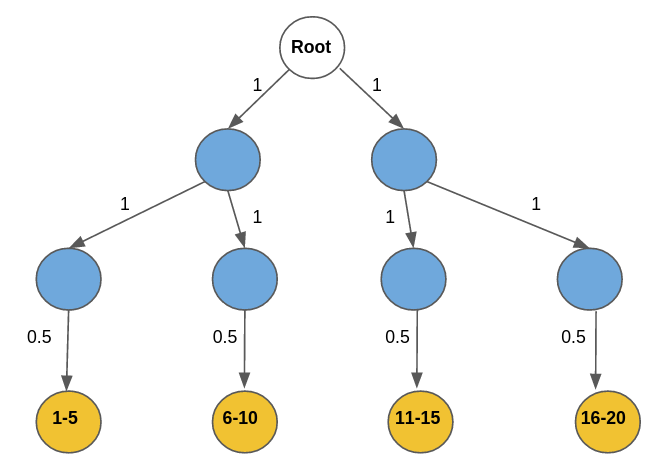
\includegraphics[scale = 0.23]{./figures/synthetic_tree_2.png} &
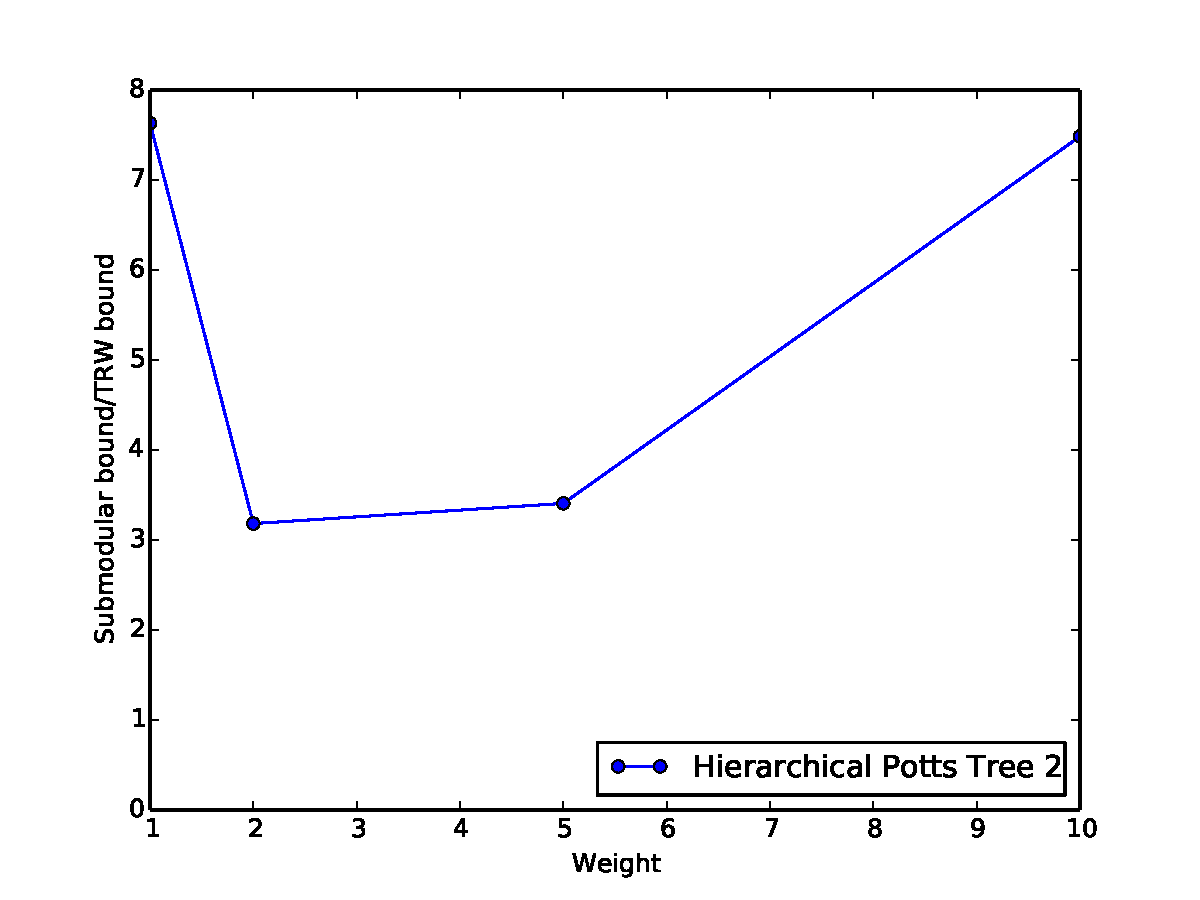
\includegraphics[scale = 0.35]{./figures/synthetic_upper_bound_tree2.pdf} \\
    \scriptsize(a)  & \scriptsize(b) \\ 
\end{tabular}
\mycaption{\footnotesize \em (a) The hierarchical Potts model defining pairwise distance among 20 labels used for upper-bound comparison with TRW. Blue nodes are the meta-labels and yellow nodes are labels. (b) Upper-bound comparison using synthetic data. The plot shows the ratio of upper bound value of log partition function from our algorithm to that of TRW averaged over 100 unary instances as a function of pairwise weights. We observe that our method results in comparable upper bound values to TRW.}
%\label{fig:syn_plot}
\end{figure*}


\mysubsection{Upper-bound Comparison using Synthetic Data with Different Tree}
%\label{subsec:synthetic}
\myparagraph{Data}  We consider hierarchical Potts model with pairwise distance between labels given by the tree of figure \ref{fig:syn_plot} (a). We vary the pairwise weight in the range $\{1, 2, 5, 10\}$. The rest of the setting is same as in the sythetic results subsection of the main paper.

\myparagraph{Method} We use the same method as described in the sythetic results subsection of the main paper. 

\myparagraph{Results} We plot the ratio of upper bound values of our method to that of TRW as a function of pairwise weights. The ratios are averaged over 100 instances of unaries. Figure \ref{fig:syn_plot} (b) shows the plots for hierarchical Potts models for the new tree. Similar to the first tree (in main paper), we find that our algorithm results in similar range of upper bound as TRW, thereby providing further empirical justification of our method.

\begin{figure*}[!]
	\centering
\begin{tabular}{ccc}
        \includegraphics[scale = 0.25]{\imagePath/stereo/venus_left} &
        \includegraphics[scale = 0.25]{\imagePath/stereo/potts/venus_left_mf_marginals} &
        \includegraphics[scale = 0.25]{\imagePath/stereo/potts/venus_left_submod_marginals} \\
        \scriptsize(a) Venus left image & \scriptsize(b) MF entropy & \scriptsize(c) Submod entropy \\
    %
        \includegraphics[scale = 0.30]{\imagePath/stereo/tsukuba_left} &
        \includegraphics[scale = 0.30]{\imagePath/stereo/potts/tsukuba_left_mf_marginals} &
        \includegraphics[scale = 0.30]{\imagePath/stereo/potts/tsukuba_left_submod_marginals} \\
        \scriptsize(a) Tsukuba left image & \scriptsize(b) MF entropy & \scriptsize(c) Submod entropy\\
         \includegraphics[scale = 0.25]{\imagePath/stereo/cones_left} &
        \includegraphics[scale = 0.25]{\imagePath/stereo/potts/cones_left_mf_marginals} &
        \includegraphics[scale = 0.25]{\imagePath/stereo/potts/cones_left_submod_marginals} \\
        \scriptsize(a) Cones left image & \scriptsize(b) MF entropy & \scriptsize(c) Submod entropy \\ 
        %
       %
         \includegraphics[scale = 0.26]{\imagePath/stereo/teddy_left} &
        \includegraphics[scale = 0.26]{\imagePath/stereo/potts/teddy_left_mf_marginals} &
        \includegraphics[scale = 0.26]{\imagePath/stereo/potts/teddy_left_submod_marginals} \\
        \scriptsize(a) Teddy left image & \scriptsize(b) MF entropy & \scriptsize(c) Submod entropy\\
\end{tabular}
\vspace{2mm}
\mycaption{\footnotesize \em Entropy plots for stereo matching using dense CRFs with Potts compatibility and Gaussian pairwise potentials for the mean-field algorithm of \citet{koltun2011efficient} and our method. We observe that our method gives more detailed uncertainty information.} 
%\label{fig:potts_entropy}
\end{figure*}

\mysubsection{Entropy Plots for Stereo Matching using Dense CRFs with Potts Model}
We plotted the entropy of the marginals obtained from mean-field and our inference algorithm for the Potts models for all the stereo matching instances. We observe that our mean-field does not give enough uncertainty information, whereas our method gives much more detailed information. However, we also observe that whereas mean-field is too certain (has less entropy) almost everywhere, our method results in uncertainty even in those regions where we expect good marginals to be certain, such as in the interior regions of objects. 

\begin{figure*}[!]
    \centering
    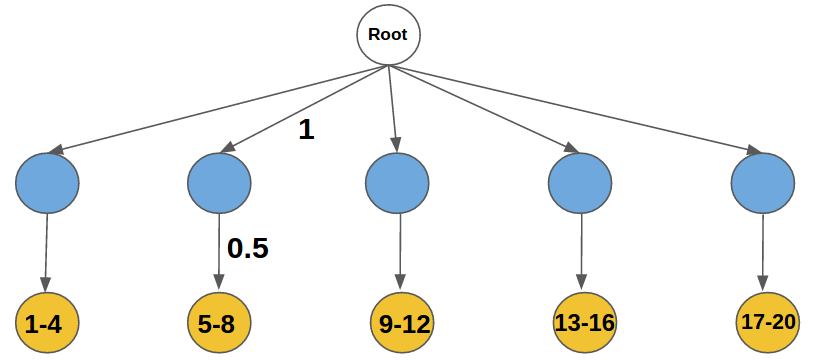
\includegraphics[scale = 0.33]{./figures/synthetic_tree.png}
    \mycaption{\footnotesize \em Tree used to specify hierachical Potts potentials for stereo matching for `Venus' image having disparity values 1-20. Similar tree topology was used for the other images.}
    %\label{fig:stereo_tree}
\end{figure*}


%==> cones_left_cones_tree1_mf.txt <==
%46.3463 3.72918e+06
%
%==> teddy_left_teddy_tree1_mf.txt <==
%62.7843 2.45632e+06
%
%==> tsukuba_left_tsukuba_tree1_mf.txt <==
%5.59413 846057
%
%==> venus_left_venus_tree1_mf.txt <==
%14.3497 1.87249e+06
%
%==> cones_left_cones_tree1_submod_tree.txt <==
%2100.14 2.62802e+07
%
%==> teddy_left_teddy_tree1_submod_tree.txt <==
%2191.12 3.46133e+07
%
%==> tsukuba_left_tsukuba_tree1_submod_tree.txt <==
%359.85  6.60389e+06
%
%==> venus_left_venus_tree1_submod_tree.txt <==
%712.88  1.55201e+07

\begin{figure*}[!]
	\centering
\begin{tabular}{ccc}
        \includegraphics[scale = 0.25]{\imagePath/stereo/venus_GT} &
        \includegraphics[scale = 0.25]{\imagePath/stereo/tree/venus_left_venus_tree1_mf} &
        \includegraphics[scale = 0.25]{\imagePath/stereo/tree/venus_left_venus_tree1_submod} \\ 
        \scriptsize(a) Venus GT & \scriptsize(b) MF solution & \scriptsize(c) Submod solution \\ 
        {} & \scriptsize 14.35 {\bf 1.87e+06} &  \scriptsize 712.88  15.52e+07\\ 
 
     
        \includegraphics[scale = 0.30]{\imagePath/stereo/tsukuba_GT} &
        \includegraphics[scale = 0.30]{\imagePath/stereo/tree/tsukuba_left_tsukuba_tree1_mf} &
        \includegraphics[scale = 0.30]{\imagePath/stereo/tree/tsukuba_left_tsukuba_tree1_submod} \\
        \scriptsize(a) Tsukuba GT & \scriptsize(b) MF solution & \scriptsize(c) Submod solution\\
        {} & \scriptsize 5.59 {\bf 0.85e+06} & \scriptsize 359.85  6.60e+06\\


        \includegraphics[scale = 0.25]{\imagePath/stereo/cones_GT} &
        \includegraphics[scale = 0.25]{\imagePath/stereo/tree/cones_left_cones_tree1_mf} &
        \includegraphics[scale = 0.25]{\imagePath/stereo/tree/cones_left_cones_tree1_submod} \\
        \scriptsize(a) Cones GT & \scriptsize(b) MF solution & \scriptsize(c) Submod solution \\
        {} & \scriptsize 46.34 {\bf 3.73e+06} &  \scriptsize 2100.14 26.28e+06\\ 
         
        
        \includegraphics[scale = 0.26]{\imagePath/stereo/teddy_GT} &
        \includegraphics[scale = 0.26]{\imagePath/stereo/tree/teddy_left_teddy_tree1_mf} &
        \includegraphics[scale = 0.26]{\imagePath/stereo/tree/teddy_left_teddy_tree1_submod} \\
        \scriptsize(a) Teddy GT & \scriptsize(b) MF solution & \scriptsize(c) Submod solution\\
        {} & \scriptsize 62.78 {\bf 2.46e+06} & \scriptsize 2191.12 34.63e+06\\
        
\end{tabular}

\mycaption{\footnotesize \em Stereo matching using dense CRFs with hierarchical Potts compatibility given by trees similar to figure \ref{fig:stereo_tree} and Gaussian pairwise potentials. We compare our solution with the mean-field algorithm of \citet{koltun2011efficient}. We observe that our method gives better-looking solutions, though mean-field runs faster and results in lower energy solutions.}
%\label{fig:stereo_hier}
\end{figure*}

\begin{figure*}[!]
	\centering
\begin{tabular}{ccc}
        \includegraphics[scale = 0.25]{\imagePath/stereo/venus_left} &
        \includegraphics[scale = 0.25]{\imagePath/stereo/tree/venus_left_venus_tree1_mf_marginals} &
        \includegraphics[scale = 0.25]{\imagePath/stereo/tree/venus_left_venus_tree1_submod_marginals} \\ 
        \scriptsize(a) Venus left image & \scriptsize(b) MF entropy & \scriptsize(c) Submod entropy \\ 
     
        \includegraphics[scale = 0.30]{\imagePath/stereo/tsukuba_left} &
        \includegraphics[scale = 0.30]{\imagePath/stereo/tree/tsukuba_left_tsukuba_tree1_mf_marginals} &
        \includegraphics[scale = 0.30]{\imagePath/stereo/tree/tsukuba_left_tsukuba_tree1_submod_marginals} \\
        \scriptsize(a) Tsukuba left image & \scriptsize(b) MF entropy & \scriptsize(c) Submod entropy\\

        \includegraphics[scale = 0.25]{\imagePath/stereo/cones_left} &
        \includegraphics[scale = 0.25]{\imagePath/stereo/tree/cones_left_cones_tree1_mf_marginals} &
        \includegraphics[scale = 0.25]{\imagePath/stereo/tree/cones_left_cones_tree1_submod_marginals} \\
        \scriptsize(a) Cones left image & \scriptsize(b) MF entropy & \scriptsize(c) Submod entropy \\
        
        \includegraphics[scale = 0.26]{\imagePath/stereo/teddy_left} &
        \includegraphics[scale = 0.26]{\imagePath/stereo/tree/teddy_left_teddy_tree1_mf_marginals} &
        \includegraphics[scale = 0.26]{\imagePath/stereo/tree/teddy_left_teddy_tree1_submod_marginals} \\
        \scriptsize(a) Teddy left image & \scriptsize(b) MF entropy & \scriptsize(c) Submod entropy\\
\end{tabular}

\mycaption{\footnotesize \em Entropy plots for stereo matching using dense CRFs with hiearchical Potts compatibility given by trees similar to figure \ref{fig:stereo_tree} and Gaussian pairwise potentials for the mean-field algorithm of \citet{koltun2011efficient} and our method. We observe that our method gives more detailed uncertainty information.}
%\label{fig:stereo_hier}
\end{figure*}

\mysubsection{Stereo Matching using Dense CRFs with Hierarchical Potts}
%\label{subsec:stereo_hier}

\myparagraph{Data} We demonstrate the benefit our algorithm for stereo matching using hierarchical Potts model. Similar to Potts case, we use images extracted from the Middlebury stereo matching dataset \citep{scharstein2001taxonomy}. We use dense CRF models with hierarchical Potts compatibility term and Gaussian pairwise potentials. The hierarchical Potts was specified using tree similar to figure \ref{fig:stereo_tree} for all images. The unary terms are obtained using the absolute difference matching function of \citep{scharstein2001taxonomy}. 

\myparagraph{Method} We used the implementation of mean-field algorithm for dense CRFs of \citep{koltun2011efficient} as our baseline. For our algorithm, we made use of the modified Gaussian filtering implementation for dense CRFs by \citep{ajanthan2017efficient} to compute the conditional gradient at each step. The step size $\gamma$ at each iteration was selected by doing line search. We ran our algorithm till 100 iterations, since the visual quality of the solution did not show much improvement beyond this point. We ran mean-field up to convergence, with a threshold of 0.001 for change in KL-divergence.

\myparagraph{Results}

Figure \ref{fig:stereo_hier} shows the solutions obtained by picking the label with maximum marginal probability for each variable for mean-field and for our algorithm. We also report the time and energy values of the solution for both methods. Though we are not performing MAP estimation, energy values give us a quantitative indication of the quality of solutions. We observe that our algorithm results in more natural looking stereo matching results. However, mean-field gives lower energy value solutions and runs faster than our method for each instance.
\fi
\clearpage
